\documentclass[sigconf,anonymous,review]{acmart}

\AtBeginDocument{%
  \providecommand\BibTeX{{Bib\TeX}}}

%% Fill in with real rights info once received from ACM / AINTEC organizers.
\setcopyright{acmlicensed}
\copyrightyear{2026}
\acmYear{2026}
\acmDOI{XXXXXXX.XXXXXXX}
\acmConference[AINTEC '26]{Asian Internet Engineering Conference}{2026}{Thailand}
\acmISBN{978-1-4503-XXXX-X/2026/XX}


\begin{document}

\title{Internet Landscape Study of Southeast Asian Countries}

\author{Anonymous}
\affiliation{%
  \institution{Anonymous Institution}
  \city{Anonymous City}
  \country{Anonymous Country}
}

\renewcommand{\shortauthors}{Anonymous}

\begin{abstract}
National Internet broadband service providers, particularly in Thailand, are
often judged from user experiences rather than systematic measurement. In
Southeast Asia this assumption remains largely unstudied. For example,
Thailand ranked 12th worldwide for fixed broadband in Ookla's Speedtest
Global Index (June 2026), yet whether such services reflect
application-level performance across the country is unclear. A 2023 survey
by the Thailand Consumer Council found that 81\% of 2,924 respondents had
encountered connection problems, mostly slow and dropping connections. These
numbers contradict each other for Thailand, and Thailand is not alone in
this mismatched information across the Southeast Asian region.

In this study we analyze and evaluate the communication network quality of
nine countries --- Thailand, Vietnam, Laos, Myanmar, Cambodia, Indonesia,
the Philippines, Malaysia, and Singapore --- using test results from Q1 2023
to Q4 2025, drawn from open datasets from Ookla (229.4 million tests) and
M-Lab NDT7 (760.6 million tests). We compare the results against the
bandwidth requirements of four popular application types: voice, video
streaming (HD), video streaming (UHD), and cloud gaming.
\end{abstract}

\keywords{Speed tests analysis, Ookla, NDT7}

\maketitle

\section{Introduction}
National Internet Service Providers (ISPs), particularly in Southeast Asian
countries like Thailand, are frequently judged based on subjective end-user
perceptions rather than systematic empirical data. A significant gap exists
between high-level speed index rankings and actual user experiences; for
example, while Thailand was ranked 12th worldwide for fixed broadband in
Ookla's Speedtest Global Index in June 2026, a 2023 survey by the Thailand
Consumer Council revealed that 81\% of 2,924 respondents suffered from
frequent connection problems such as slow speeds and dropped signals. To
address this widespread mismatch across the region, this paper presents a
comprehensive study analyzing communication network quality across nine
Southeast Asian nations: Thailand, Vietnam, Laos, Myanmar, Cambodia,
Indonesia, the Philippines, Malaysia, and Singapore. Leveraging
cross-platform open measurement datasets collected from Q1 2023 to Q4
2025 --- comprising 229.4 million tests from Ookla and 760.6 million tests
from Measurement Lab's NDT7 --- we evaluate performance against real-world
application demands. By establishing bandwidth and latency threshold
requirements for four primary application types (voice, HD video streaming,
Ultra HD video streaming, and cloud gaming), this research provides a
multi-dimensional assessment of regional fixed broadband and cellular
networks, capturing spatial inequality, ISP performance tiers, and
application-level delivery capabilities.

\section{Related Work}
This research is performed using open datasets from Ookla and Measurement
Lab (NDT7). The next subsections cover the related work for each dataset,
followed by prior work applying the same threshold-based evaluation
methodology.

\subsection{Ookla}
Ookla is a prominent publicly available crowdsourced performance platform
that serves as a primary foundation for empirical internet measurement.
Ookla Speedtest is one of the most widely deployed commercial frameworks.
Prior literature highlights key architectural and methodological
differences between platforms like Ookla and open research datasets such as
Measurement Lab (MLab). \textbf{[CITATION NEEDED] Rajabiun and McKelvey} demonstrate that Ookla
consistently reports significantly higher throughput values than MLab or
Akamai. These discrepancies stem largely from server placement: Ookla
frequently deploys measurement servers directly within access ISPs'
internal networks, whereas platforms like MLab utilize off-net servers
placed in transit networks outside the provider's domain. Consequently,
researchers note that while Ookla's approach isolatedly measures the
maximum theoretical capacity of the immediate broadband access network (the
``last mile''), off-net platforms capture broader end-to-end paths that
reflect realistic user application performance across interconnected
transit networks. \textbf{[CITATION NEEDED] Feamster and Livingood} emphasize that Ookla's engine
relies on opening multiple parallel TCP streams and excluding initial
slow-start phases, designed specifically to saturate high-speed links and
overcome minor bottleneck losses. While this multi-stream design reliably
estimates link capacity, single-stream testing methodologies as used in
standard MLab NDT provide a more realistic proxy for traditional end-user
application flows, such as web browsing or adaptive video streaming.
Additionally, Deng et al.~\cite{Deng2021} point out that user-initiated
tests like Ookla are subject to sampling bias and spatial multiplexing
distortions --- such as multiple devices operating behind Network Address
Translation (NAT) --- which require dedicated data curation protocols to
extract unbiased, longitudinal insights regarding ISP performance and
infrastructure bottlenecks.

The availability of open measurement data has expanded further through
Ookla's Open Data Initiative~\cite{OoklaOpenData2023}, which publicly
distributes aggregated global fixed and mobile network performance maps.
Unlike the raw, test-by-test measurements provided by MLab, Ookla's open
dataset aggregates consumer-initiated tests into standardized spatial tiles
using a Web Mercator projection (zoom level 16, approximately 600 m
$\times$ 600 m at the equator). This spatial aggregation provides
quarter-by-quarter metrics for average download speed, upload speed,
latency, tests conducted, and unique active devices. While this tiled data
masking mitigates raw IP-level privacy concerns and reduces data volume for
macro-level analysis, researchers emphasize that spatial aggregation
introduces a different trade-off. The open Ookla data inherently obscures
temporal granularities --- such as identifying specific peak-hour
congestion windows or evaluating protocol-level stack behaviors (e.g.,
individual TCP flow stats) --- which are accessible in unaggregated MLab
datasets. Consequently, empirical studies increasingly treat Ookla's open
spatial dataset and MLab's open granular dataset as complementary tools:
Ookla provides fine-grained geographic mapping of broadband availability,
whereas MLab offers deep longitudinal insight into end-to-end transport
protocol dynamics and busy-hour network degradation.

\subsection{Measurement Lab NDT7}
The Measurement Lab (MLab) Network Diagnostic Tool (NDT) protocol
represents a key benchmark in single-stream Internet performance
measurement, evolving significantly with the deployment of
NDT7~\cite{Gill2022}. Designed to measure single-stream ``bulk transport
capacity,'' NDT isolates the transport-layer throughput and round-trip time
(RTT) available to standard end-user applications. Older iterations of the
platform (web100 and NDT5) relied on TCP Reno and TCP Cubic protocols along
with non-standard ports, which often required administrative permissions or
specialized client setups. In contrast, NDT7 modernizes active measurement
by running over WebSockets over TLS via standard HTTP(S) ports (80/443).
This shift significantly expands client browser compatibility, eliminates
middlebox port-filtering artifacts, and simplifies third-party measurement
integrations without compromising network diagnostics.

A core advancement of NDT7 is its native integration of the TCP BBR
(Bottleneck Bandwidth and Round-trip propagation time) congestion control
algorithm, which replaces loss-based algorithms like Cubic where supported.
By continuously estimating bottleneck bandwidth and minimum RTT, BBR
actively prevents queue buildup in intermediate buffers. In empirical
studies, NDT7 measurements show a substantial reduction in self-induced
bufferbloat, yielding lower, more accurate baseline latency metrics
compared to older single-stream tests. Researchers emphasize that NDT7
provides a much more faithful reflection of modern web traffic behavior and
realistic user application performance across interconnected broadband
networks.

\subsection{The German Internet Landscape}
Prior research by L\"ubben and Misfeld~\cite{Lubben2022} investigates the
state of Germany's Internet performance by analyzing the Measurement Lab
(MLab) open dataset using Network Diagnostic Tool (NDT) active test data
collected between January 2019 and August 2021. The authors highlight how
open broadband datasets --- despite originating from user-initiated,
uncontrolled environments --- can yield remarkably reliable insights into
end-to-end network quality and application support capabilities when
subjected to rigorous data curation. By isolating busy hours (8 p.m. to
10 p.m.), accounting for repeated measurements per IP, and controlling for
server locations and TCP congestion control protocols, the methodology
demonstrates that open data can effectively evaluate real-world application
performance. The study uses these end-to-end measurements to assess whether
current networks meet the high bandwidth and low latency demands of modern
services like HD/UHD video streaming and cloud gaming. The bandwidth and
latency requirements for different types of applications are used as a
threshold to evaluate whether services are good enough for such
applications, a methodology we adopt in Table~\ref{tab:app-requirements}.

\begin{table}
  \caption{Bandwidth and latency requirements for different types of applications}
  \label{tab:app-requirements}
  \begin{tabular}{lll}
    \toprule
    Application Type & Required Data Rate & Required Latency \\
    \midrule
    Voice                    & 64 Kbps & 200 ms \\
    Video Streaming (HD)     & 5 Mbps  & few secs \\
    Video Streaming (UHD)    & 25 Mbps & few secs \\
    Cloud Gaming             & 44 Mbps & 25 ms \\
    \bottomrule
  \end{tabular}
\end{table}

\section{Datasets}
Ookla open data supplies quarterly internet-performance tiles split by
connection type (fixed, mobile) at Quadkey zoom 16
($\sim$600$\times$600 m), each carrying mean download, upload, latency, and
the underlying Speedtest submission count, delivered as global Parquet
files on Amazon S3. We map them to the nine countries and twelve quarters
(Q1 2023--Q4 2025), giving a total of 229{,}367{,}221 tests, with the
largest Indonesia test data of 74.2 million records and the smallest Laos
dataset of 875{,}799 records.

Total volume across the nine countries from MLab NDT7 is 760{,}607{,}387
tests, with the largest Indonesia test data of 367.2 million and the
smallest Laos test record of 139{,}693 records.

\section{Data Cleansing and Preparation}
The data from the two sources comes in different formats. Ookla comes as
spatial tiles approximately 600 m $\times$ 600 m, while NDT7 comes as
individual test records. We analyze the data separately as well as
together. First, we clean the data by removing records with throughput
$\leq 0$ and duration $\leq 0$. We then use ip-api.com~\cite{IpApi}, a free
API service, to check whether test records carry mobile/hosting/proxy flags
and to resolve the ASN for each IP.

To use both data sources together, we preprocess the NDT7 dataset into
tiles like those from Ookla using GeoPandas~\cite{GeoPandas2020} and
Shapely, performing a point-in-polygon join of client coordinates against
province/region boundaries, using \texttt{sjoin\_nearest} for coordinates
that fall outside every polygon (e.g., coastal points) to compute distance
for accuracy.

On the Ookla dataset, we build a bounding box to define each country's
extent, referencing the geoBoundaries ADM1 file~\cite{Runfola2020} for the
nine ASEAN countries (Thailand, Indonesia, Philippines, Vietnam, Malaysia,
Myanmar, Cambodia, Laos, Singapore), then run point-in-polygon on the tiles
to determine which province each point falls in, using each country's
GeoJSON. We then compute a weighted average by each tile's test count to
prevent distortion from tiles with widely different test counts. To ensure
quality, we filter only province-quarters with \texttt{total\_tests}
$\geq 100$ and \texttt{n\_tiles} $\geq 5$, which better represents reality.
Furthermore, we found data-completeness issues in some areas. For Vietnam
and Cambodia, mobile test data is missing in some provinces for some
quarters because these are small areas with low test counts. Myanmar is
another case: a fairly large amount of data is missing on both broadband
(10.7\%) and mobile (22\%) services.

On the MLab NDT7 dataset, we query each country's test results using
BigQuery~\cite{BigQuery}, then determine the province using
point-in-polygon referencing the GADM 4.1 file~\cite{GADM2022}. We
identified and separated mobile and fixed broadband, and separated cloud
services from individual clients. Due to ISP name spelling differences,
operators are grouped using ASN rather than M-Lab's raw ISP-name field,
which is unreliable at scale. For very large datasets, particularly
Indonesia, we needed to cut down the time required to obtain the whole
27-day dataset, so we strategically sampled the dataset in a way proven to
be a good representative of the whole. For the remaining countries we
obtained the whole dataset during the studied period.

For grouping operators, we rely primarily on the ASN (Autonomous System
Number), because ISP names from M-Lab can be outdated, and a single
operator can appear under hundreds of different name spellings. Using ASN
is therefore far more accurate.

\section{Data Analysis}
Across the nine Southeast Asian countries analyzed, Ookla fixed broadband
data (2023 Q1--2025 Q4) reveals significant regional performance tiers
alongside pronounced urban-rural divides when comparing capital city
performance against national averages. Singapore leads the region overall,
with its Central Region reaching 341 Mbps, slightly below its top national
baseline (376 Mbps). In contrast, most other capital regions significantly
outperform their nationwide benchmarks: Bangkok Metropolis leads Thailand
at 295 Mbps (vs.\ 244 Mbps national), Kuala Lumpur drives Malaysia to
210 Mbps (vs.\ 178 Mbps national), the Philippines' NCR reaches 159 Mbps
(vs.\ 106 Mbps national), and Hanoi records 153 Mbps for Vietnam (vs.\
135 Mbps national). At the lower end of the spectrum, Cambodia (Phnom Penh
at 54 Mbps vs.\ 44 Mbps national) and Laos (Vientiane Capital at 53 Mbps
vs.\ 45 Mbps national) show modest capital premiums, while Myanmar (Yangon)
trails at 27 Mbps, sitting slightly below its national average of 29 Mbps.
Overall, these metrics highlight a stark infrastructure gap where
top-performing capital hubs achieve speeds more than 12 times greater than
lower-tier regions, with metropolitan centers generally serving as the
primary drivers of national connectivity.

\begin{figure}
  \centering
  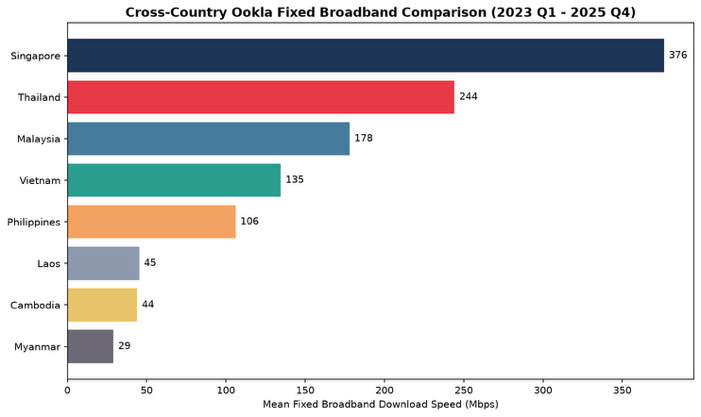
\includegraphics[width=0.48\linewidth]{figures/image1.png}
  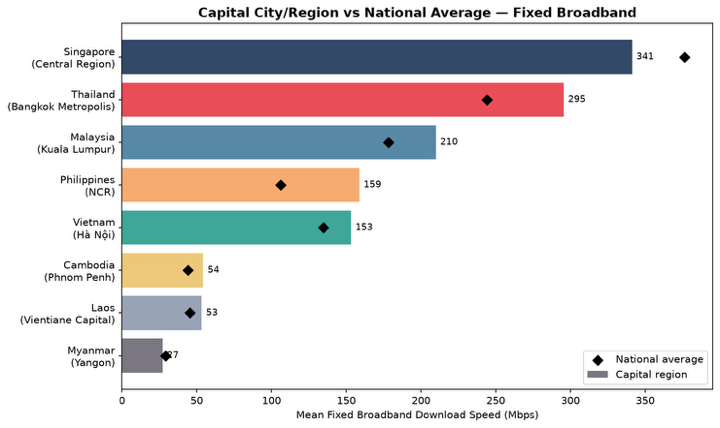
\includegraphics[width=0.48\linewidth]{figures/image2.png}
  \caption{Mean download speed of fixed broadband (Ookla)}
  \Description{Two maps showing mean download speed of fixed broadband across Southeast Asian countries.}
  \label{fig:fixed-download}
\end{figure}

The chart in Figure~\ref{fig:mobile-download} compares fixed broadband and
mobile mean download speeds across nine Southeast Asian countries,
highlighting the fixed-to-mobile performance ratio for each nation. Fixed
broadband speeds generally outperform mobile speeds across most of the
region, led by Singapore (nearly 400 Mbps fixed vs.\ $\sim$190 Mbps mobile,
a 2.1x ratio) and Thailand, which exhibits the largest disparity with fixed
speeds exceeding mobile by 3.2x ($\sim$275 Mbps vs.\ $\sim$85 Mbps).
Malaysia, Vietnam, and the Philippines follow with fixed download speeds
ranging from $\sim$130 Mbps to $\sim$195 Mbps and fixed-to-mobile ratios
between 1.1x and 1.9x. In contrast, developing markets --- including
Cambodia, Laos, Indonesia, and Myanmar --- demonstrate much lower overall
download speeds (50 Mbps) and near parity between fixed and mobile
performance (1.1x to 1.4x ratios). Notably, Myanmar is the sole outlier
where mobile download speeds actually surpass fixed broadband performance
(0.8x ratio), reflecting a mobile-first infrastructure reliance.

\begin{figure}
  \centering
  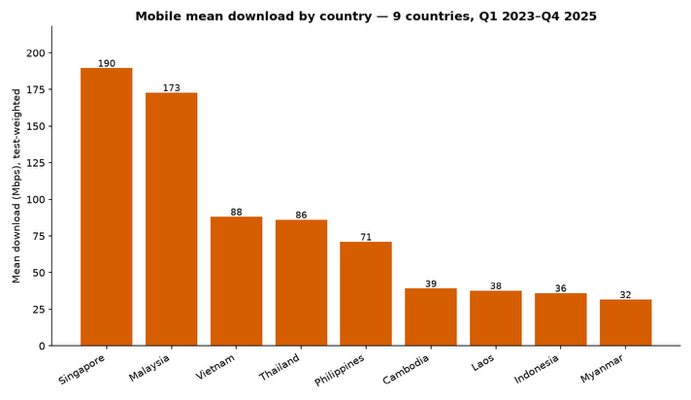
\includegraphics[width=0.48\linewidth]{figures/image3.png}
  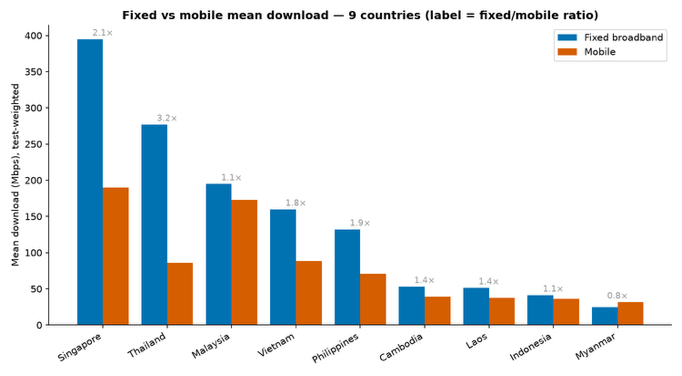
\includegraphics[width=0.48\linewidth]{figures/image4.png}
  \caption{Mean download speed of mobile and comparison to fixed (Ookla)}
  \Description{Bar charts comparing fixed and mobile mean download speeds across nine countries and their fixed-to-mobile ratios.}
  \label{fig:mobile-download}
\end{figure}

The analysis in Figure~\ref{fig:top5} shows the top five fastest provinces
or regions for fixed broadband mean download speeds across nine Southeast
Asian countries, using hatched bars to flag low-sample regions carrying
under 5\% of national tests as statistically unreliable. Singapore leads
all nations by a wide margin, with speeds exceeding 360 Mbps across all
regions, led by its North Region at 416 Mbps. In Thailand, suburban and
industrial provinces surrounding Bangkok dominate performance at over
290 Mbps, though all top five entries carry hatched markings due to low
test volumes. Malaysia and the Philippines demonstrate high speeds
concentrated in major economic hubs like Kuala Lumpur (212 Mbps) and NCR
(160 Mbps), alongside significant sample sizes. In contrast, emerging
broadband markets like Vietnam, Indonesia, Cambodia, Laos, and Myanmar
register top regional speeds below 200 Mbps --- with lower-performing
nations dropping below 70 Mbps --- and rely heavily on low-sample
provinces to fill out their top rankings.

\begin{figure}
  \centering
  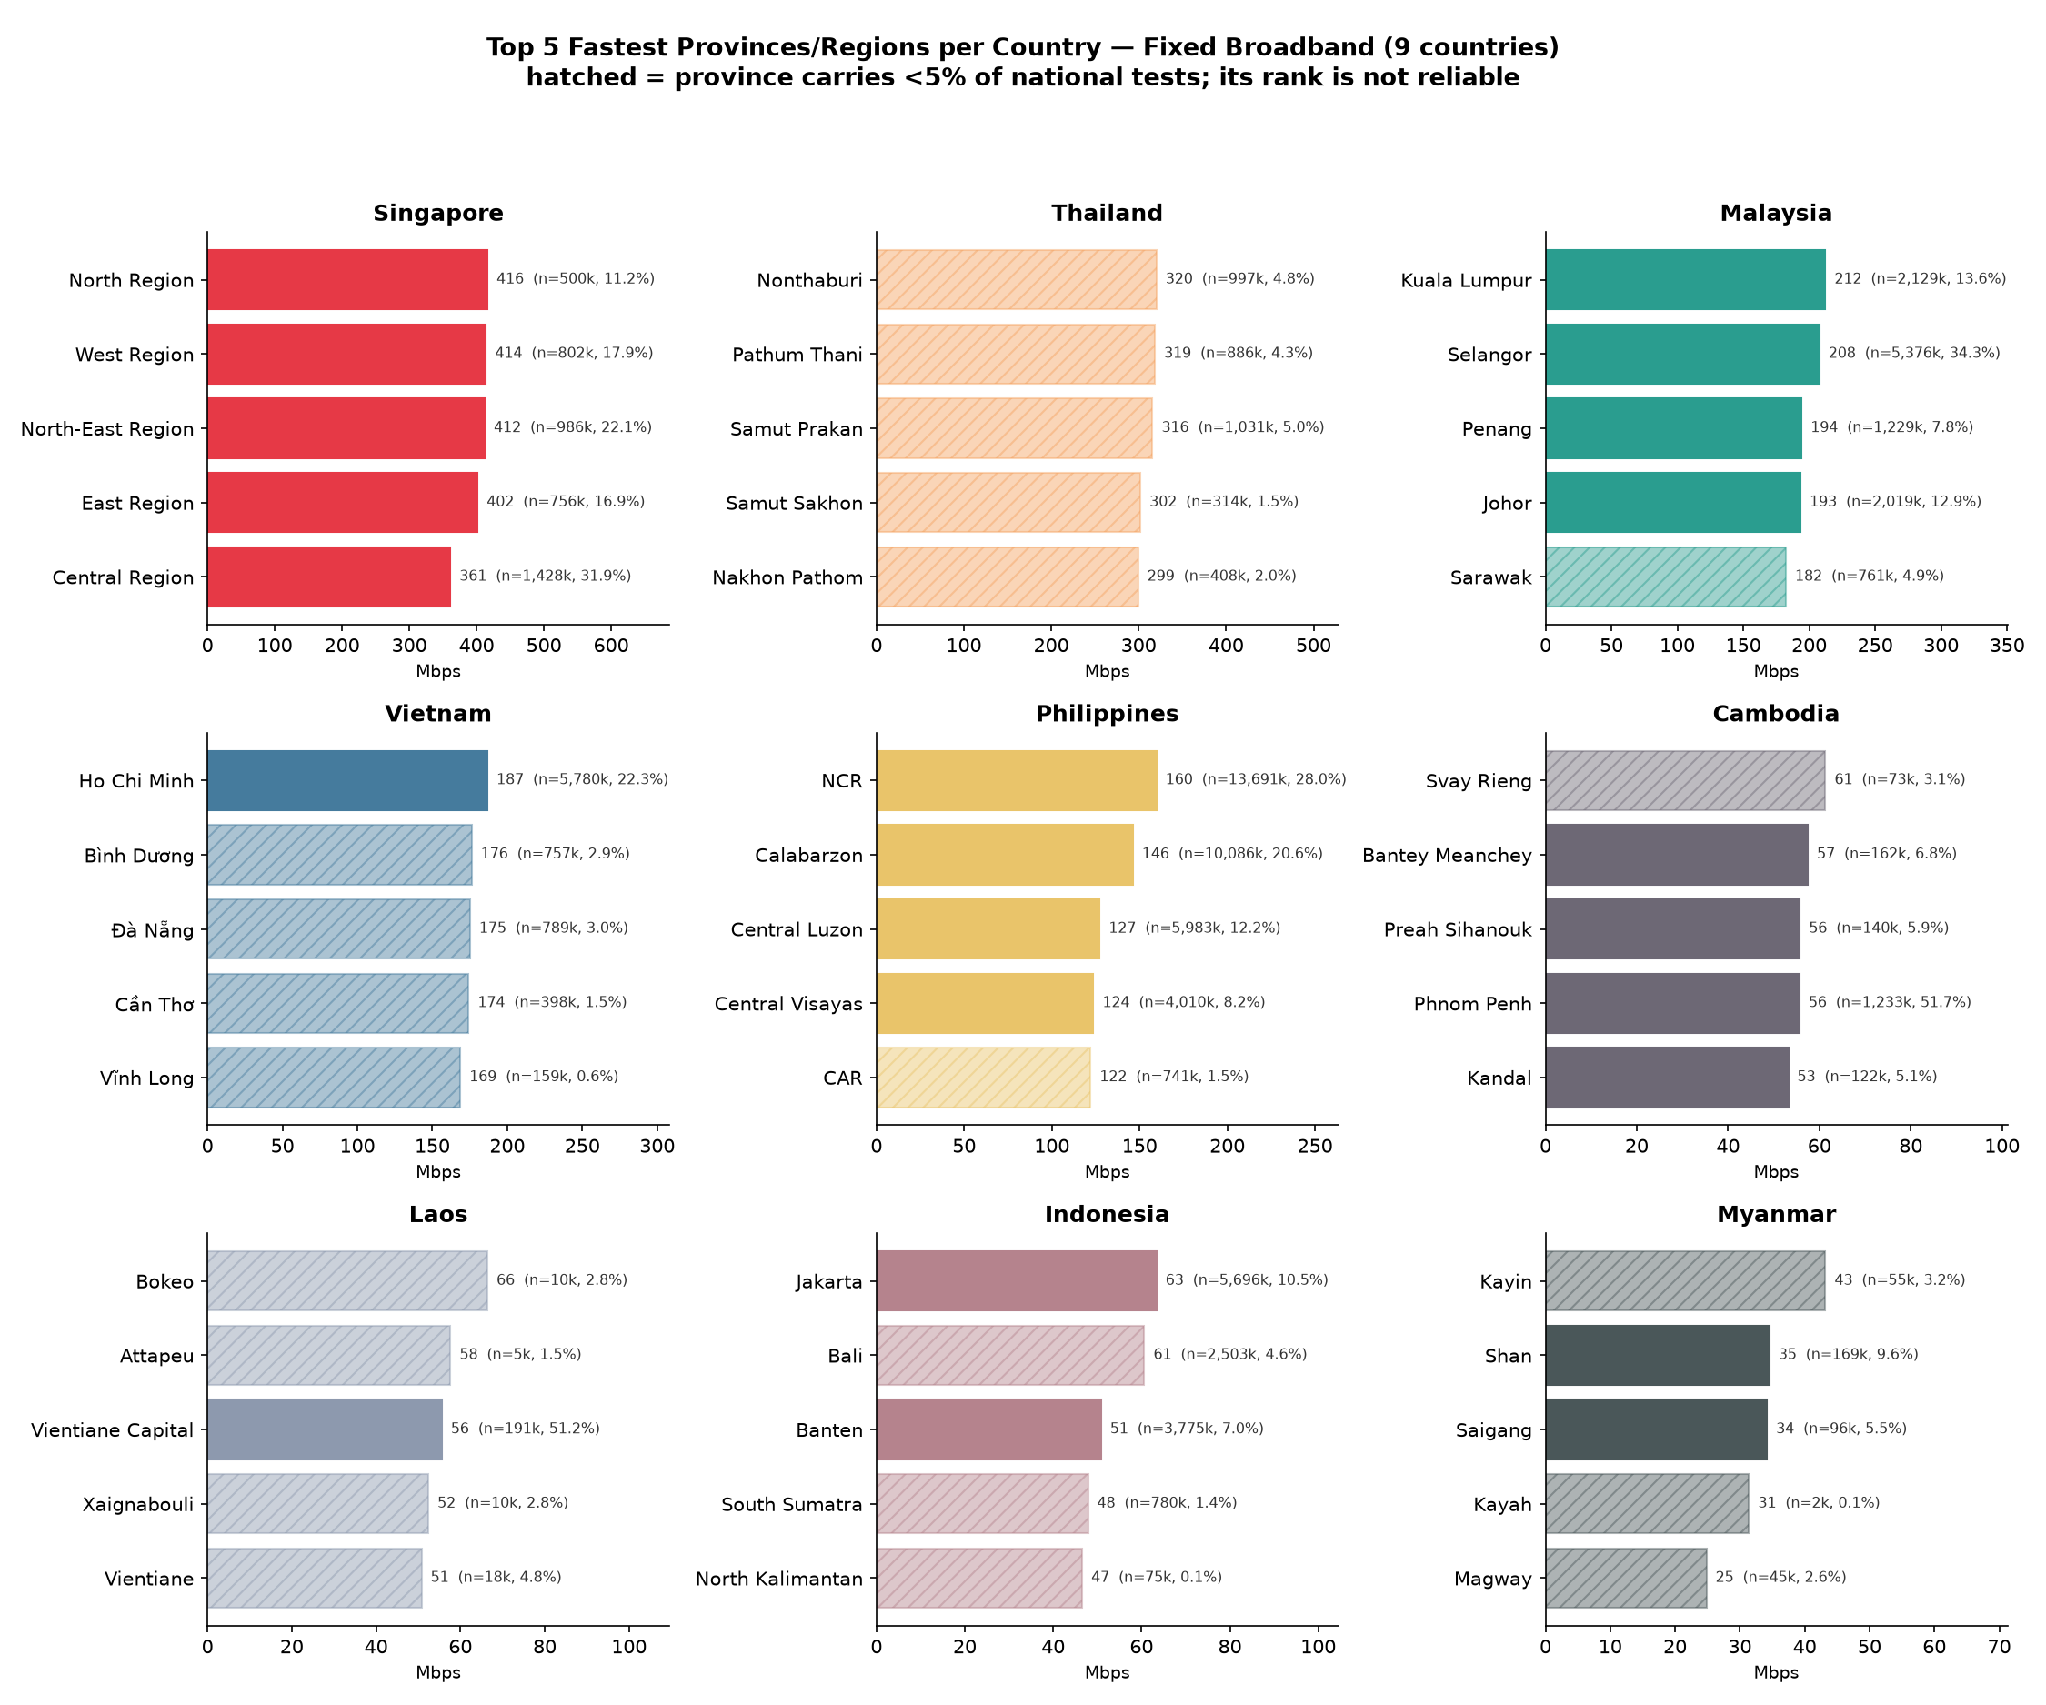
\includegraphics[width=\linewidth]{figures/image5.png}
  \caption{The top five fastest provinces of each country}
  \Description{Bar chart of the top five fastest provinces or regions for fixed broadband mean download speeds in each of the nine countries.}
  \label{fig:top5}
\end{figure}

The graph in Figure~\ref{fig:quarterly-growth} tracks the quarterly growth
of median provincial fixed broadband download speeds across nine Southeast
Asian nations from Q1 2023 through Q4 2025. Singapore demonstrates the
steepest growth trajectory by a wide margin, nearly doubling its median
provincial speed from $\sim$280 Mbps in early 2023 to nearly 550 Mbps by
late 2025. Thailand maintains a steady second position, scaling from
$\sim$200 Mbps to around 300 Mbps, while Malaysia and Vietnam form a strong
middle tier, with Vietnam showing notable acceleration to catch up to
Malaysia at over 200 Mbps by Q4 2025. The Philippines experiences moderate
growth, hovering near 100 Mbps before closing around 120 Mbps. Meanwhile,
developing broadband markets --- including Laos, Cambodia, Indonesia, and
Myanmar --- cluster tightly at the bottom, registering flat or minimal
growth under 60 Mbps throughout the entire three-year period, with Myanmar
briefly dropping near 0 Mbps at the end of 2025.

\begin{figure}
  \centering
  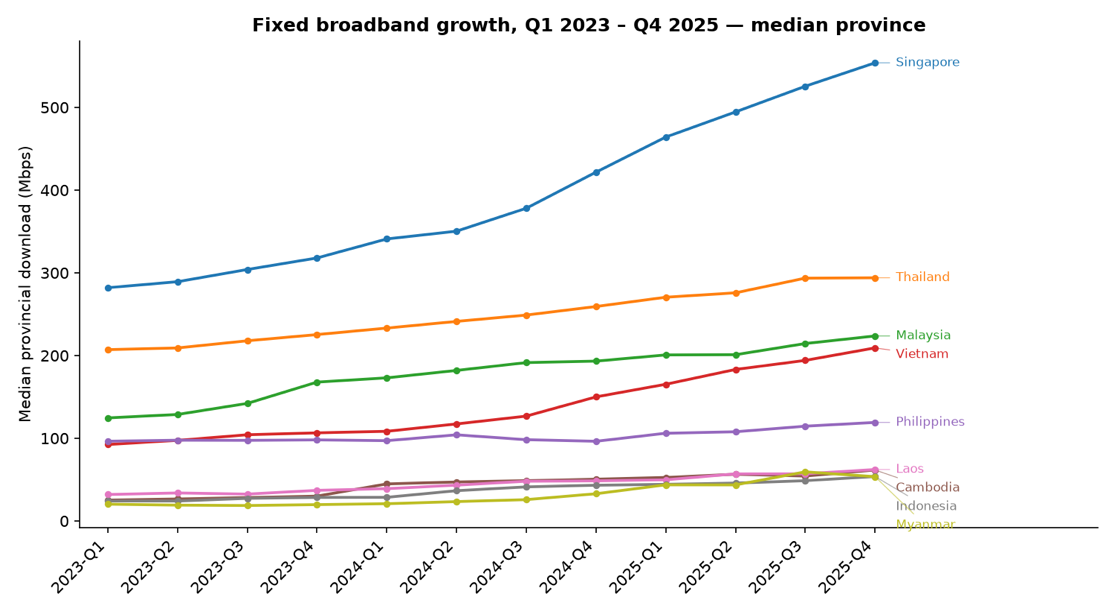
\includegraphics[width=\linewidth]{figures/image6.png}
  \caption{Quarterly growth of median provincial fixed broadband download speeds across nine Southeast Asian nations}
  \Description{Line chart tracking quarterly median provincial fixed broadband download speeds from Q1 2023 to Q4 2025.}
  \label{fig:quarterly-growth}
\end{figure}

The side-by-side bar charts in Figure~\ref{fig:fastest-operator} compare
the average download speeds of the fastest major operator (defined as
having a market share $\geq 5\%$) across Southeast Asian nations for both
fixed broadband and cellular networks. In fixed broadband, Singapore's
MyRepublic leads the region by a significant margin with an average
download speed of 300 Mbps (7\% share), followed by Malaysia's TIME dotCom
at 196 Mbps (13\% share) and Thailand's AIS at 126 Mbps (23\% share). The
remaining markets record top provider broadband speeds below 100 Mbps,
scaling down from Globe in the Philippines (90 Mbps, 12\% share) and Viettel
in Vietnam (71 Mbps, 39\% share) to low-tier performances in Indonesia
(Biznet, 43 Mbps), Laos (Unitel, 43 Mbps), Cambodia (Angkor Data
Communication, 31 Mbps), and Myanmar (Global Technology, 23 Mbps). In
cellular networks, speeds are universally lower and more compressed across
the region, though Singapore again leads with Singtel Mobile reaching
104 Mbps (37\% share), followed by Malaysia's Maxis at 53 Mbps (27\%
share). Across the remaining seven markets, cellular speeds for leading
providers tightly cluster within a narrow range between 22 Mbps and
39 Mbps --- led by Viettel in Vietnam (39 Mbps) and DITO in the Philippines
(31 Mbps), down to Unitel in Laos (22 Mbps) --- demonstrating a far smaller
cross-country disparity in mobile performance compared to fixed broadband
infrastructure.

\begin{figure}
  \centering
  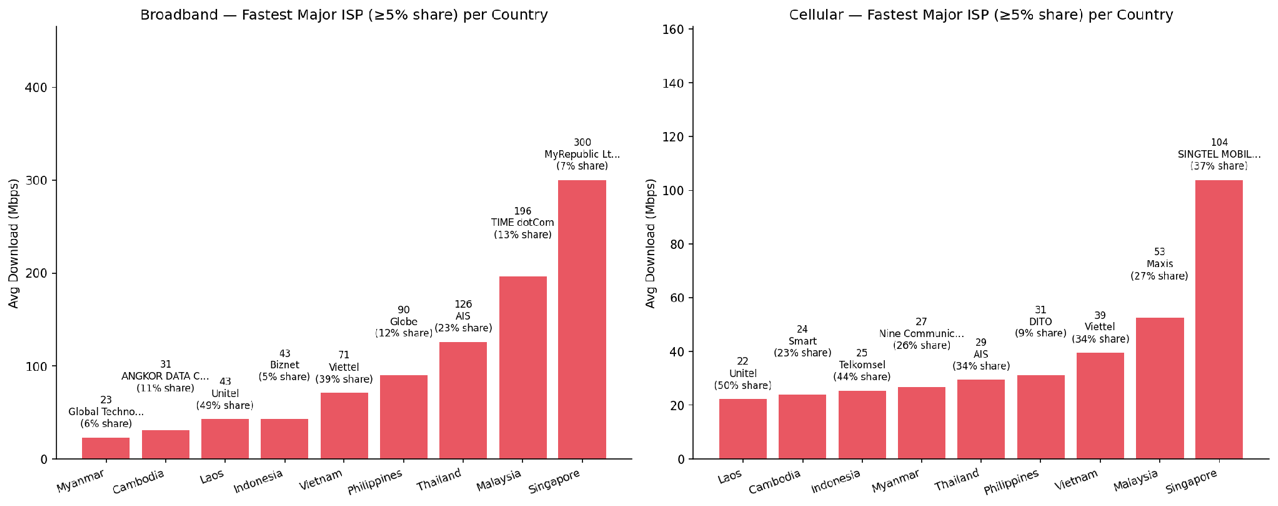
\includegraphics[width=\linewidth]{figures/image7.png}
  \caption{Comparison of the average download speeds of the fastest operators of each country}
  \Description{Bar charts comparing the fastest fixed and cellular operators per country by market share and average download speed.}
  \label{fig:fastest-operator}
\end{figure}

Figure~\ref{fig:most-used-operator} evaluates the average download speeds
of the single most-used Internet Service Provider (ISP) per country,
determined by total measurement sample volume ($n$), across both fixed
broadband and cellular networks in Southeast Asia. For fixed broadband,
market dominators show vast performance disparities across the region:
Singtel Fibre Broadband in Singapore leads significantly at 176 Mbps
($n$=2.6M), followed by Thailand's True at 115 Mbps ($n$=5.8M) and
Malaysia's TM at 113 Mbps ($n$=1.1M). Mid-tier market leaders include
Viettel in Vietnam (71 Mbps, $n$=4.4M) and PLDT in the Philippines
(61 Mbps, $n$=48.6M), while the most-used broadband providers in
lower-tier markets deliver substantially lower speeds, ranging from Unitel
in Laos (43 Mbps) and Metfone in Cambodia (30 Mbps) down to Telkom
Indonesia (19 Mbps, $n$=67.2M) and Mytel in Myanmar (10 Mbps). In cellular
networks, download speeds for primary operators display a much tighter
regional distribution, with the exception of Singapore, where Singtel
Mobile achieves a dominant 104 Mbps ($n$=841k). Across all other eight
nations, the most-used cellular providers deliver average speeds within a
narrow band between 19 Mbps and 45 Mbps. U Mobile in Malaysia leads this
non-Singapore group at 45 Mbps ($n$=408k), followed by Viettel in Vietnam
(39 Mbps, $n$=196k), Telkomsel in Indonesia (25 Mbps, $n$=23.4M), MPT in
Myanmar (25 Mbps), Unitel in Laos (22 Mbps), Smart in the Philippines
(21 Mbps, $n$=19.0M), True in Thailand (20 Mbps, $n$=5.8M), and Metfone in
Cambodia (19 Mbps, $n$=104k). Overall, the data illustrates that while
dominant fixed broadband performance varies wildly across national
markets, widely adopted cellular networks offer far more uniform baseline
capabilities across Southeast Asia.

\begin{figure}
  \centering
  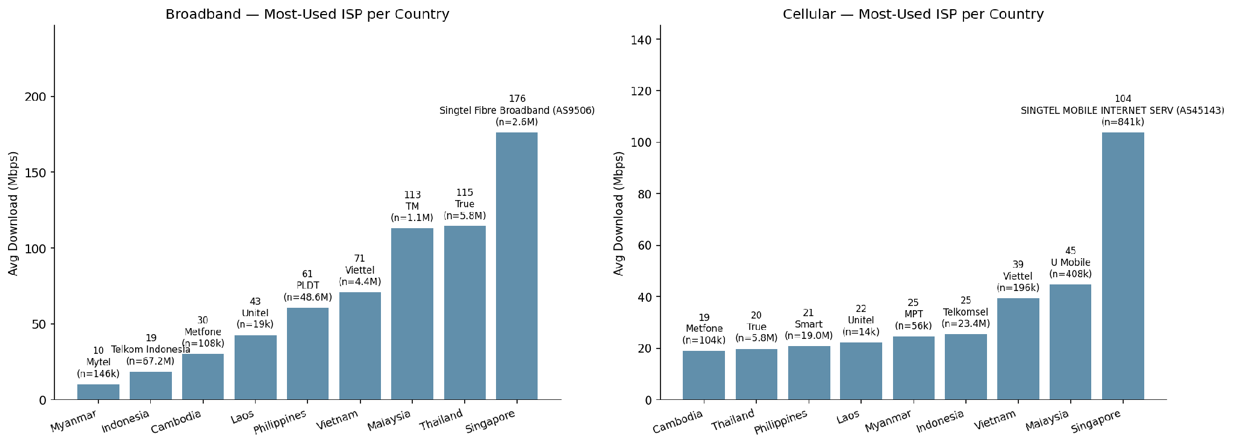
\includegraphics[width=\linewidth]{figures/image8.png}
  \caption{Comparison of the average download speeds of the major operators of each country}
  \Description{Bar charts comparing the most-used fixed and cellular operators per country by sample volume and average download speed.}
  \label{fig:most-used-operator}
\end{figure}

Figure~\ref{fig:app-eval} shows the evaluation results against the
application requirements from Table~\ref{tab:app-requirements}.

\begin{figure}
  \centering
  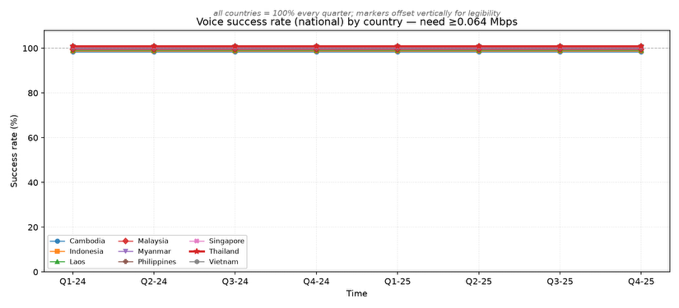
\includegraphics[width=0.48\linewidth]{figures/image9.png}
  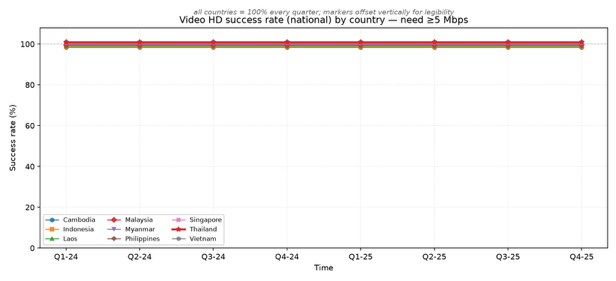
\includegraphics[width=0.48\linewidth]{figures/image10.png}\\[2mm]
  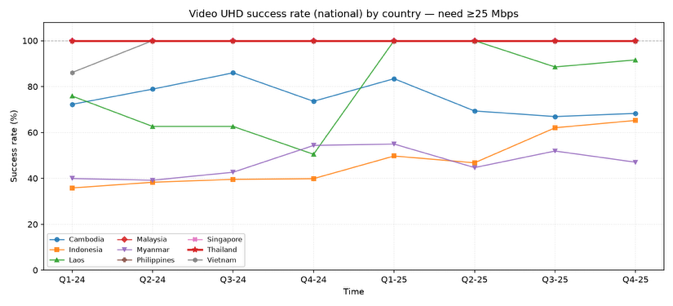
\includegraphics[width=0.48\linewidth]{figures/image11.png}
  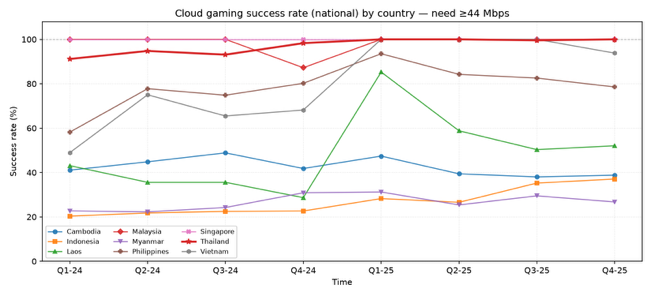
\includegraphics[width=0.48\linewidth]{figures/image12.png}
  \caption{Evaluation results on the application requirements}
  \Description{Four line charts showing national success rates over time for voice, HD video, UHD video, and cloud gaming thresholds.}
  \label{fig:app-eval}
\end{figure}

For the national-level success rate for voice and HD video streaming ---
defined as achieving a download speed of $\geq$ 64 Kbps and 5 Mbps
respectively --- across nine Southeast Asian countries from Q1 2024 through
Q4 2025, every single country consistently achieves a 100\% success rate
every quarter, with the trendlines remaining entirely flat and parallel
near the top of the scale (offset slightly purely for visual legibility).
This indicates that across all evaluated nations, including lower-tier
broadband markets, existing fixed and mobile network infrastructure
universally meets the basic 5 Mbps threshold required for smooth HD video
playback without performance bottlenecks. However, the national success
rates for Ultra High Definition (UHD) video streaming --- defined as
achieving download speeds of $\geq$ 25 Mbps --- across eight quarters (Q1
2024 to Q4 2025) reveal a clear divergence in performance across Southeast
Asian nations. Advanced broadband markets including Malaysia, Singapore,
Thailand, the Philippines, and Vietnam consistently achieve a 100\% success
rate throughout the entire period (clustering together along the top
boundary). In contrast, developing markets exhibit lower and more volatile
success rates: Laos shows significant fluctuation, climbing from
$\sim$76\% in Q1 2024, dipping to 50\% in Q4 2024, surging to 100\% in Q1
2025, and stabilizing around 92\% by Q4 2025. Cambodia maintains moderate
success rates fluctuating between 67\% and 86\%, while Indonesia
demonstrates steady upward progress from $\sim$36\% to 65\%. Myanmar
consistently trails the region, with its UHD success rate hovering between
40\% and 55\% over the two-year timeframe, illustrating that higher
bandwidth requirements like UHD video continue to expose infrastructure
constraints in emerging digital economies. Additionally, the national
success rates for cloud gaming --- defined by a demanding bandwidth
threshold of $\geq$ 44 Mbps --- across nine Southeast Asian nations from Q1
2024 to Q4 2025 show Singapore, Thailand, and Malaysia forming the top
tier, with Singapore maintaining a near-perfect 100\% success rate
throughout, while Thailand and Malaysia fluctuate slightly around
87\%--100\%. The Philippines and Vietnam occupy a mid-tier position;
Vietnam shows dramatic improvement from under 50\% in Q1 2024 to peaking at
100\% in Q1 2025 before settling around 94\%, while the Philippines ranges
between 58\% and 93\%. In contrast, lower-tier markets face severe
bottlenecks meeting this intensive threshold: Cambodia hovers between 38\%
and 49\%, Laos surges briefly to 85\% in early 2025 before dropping back to
$\sim$52\%, and Indonesia and Myanmar consistently trail the region at the
bottom, struggling below 38\% and 31\% success rates, respectively.

Taken together, these findings demonstrate that while basic connectivity
needs like HD video streaming $\geq$ 5 Mbps are universally met across
Southeast Asia, substantial performance disparities persist when evaluating
higher bandwidth demands, spatial distribution, and end-to-end application
capabilities. Fixed broadband performance exhibits a severe regional
divide --- led by Singapore and Thailand --- with high speeds heavily
concentrated in primary capital hubs and major economic centers. While
mobile networks offer a more uniform and accessible baseline across
emerging markets like Myanmar, Laos, and Cambodia, they struggle to bridge
the gap for data-intensive, low-latency applications. As bandwidth
requirements scale to Ultra High Definition video $\geq$ 25 Mbps and cloud
gaming $\geq$ 44 Mbps, infrastructure bottlenecks in developing nations
become glaringly evident. Ultimately, this empirical analysis highlights
the critical need for continued fiber expansion and transport-layer
optimizations to narrow the digital divide and support next-generation
digital services across the region.

\section{Conclusion}
This study provides a multi-year empirical evaluation of network
infrastructure performance and application readiness across nine Southeast
Asian nations using over 990 million tests from Ookla and M-Lab NDT7
datasets. Our findings reveal that while foundational network
requirements --- such as voice calls and HD video streaming $\geq$ 5 Mbps ---
are universally met with a 100\% success rate across all evaluated
countries, significant digital divides emerge under higher-tier demands.
Fixed broadband infrastructure exhibits stark regional stratification and
severe urban-rural disparities, with primary capital hubs achieving speeds
up to 12 times higher than lower-tier regions. While mobile networks
provide a more spatially uniform and reliable baseline in developing
economies like Myanmar, Laos, and Cambodia, they struggle to sustain
bandwidth-intensive, latency-critical workloads. As network requirements
scale to Ultra HD streaming $\geq$ 25 Mbps and cloud gaming $\geq$ 44 Mbps,
performance diverges sharply: tier-one markets like Singapore, Thailand,
and Malaysia consistently deliver seamless execution, whereas developing
markets face severe infrastructural bottlenecks that drop success rates
below 38\%. Ultimately, this research underscores that raw speed rankings
fail to reflect end-to-end user experiences across diverse application
types, highlighting the imperative for targeted fiber deployment, regional
infrastructure investments, and transport-layer optimizations to achieve
true digital equity across Southeast Asia.

\section*{Ethics and Privacy Statement}
This study relies exclusively on publicly available, already-aggregated or
anonymized open datasets (Ookla Open Data, M-Lab NDT7 via BigQuery) and
does not collect any new data from individuals. IP addresses used
transiently for ASN/geolocation resolution via ip-api.com are not
retained. We do not foresee societal risks beyond those already considered
by the dataset providers' own privacy safeguards.

\bibliographystyle{ACM-Reference-Format}
\bibliography{references}

\end{document}
